\chapter{Modelagem de Turbulência}\label{cap:turbulencia}
\graphicspath{{chapter-04/img-cap04/}}

No âmbito da modelagem de turbulência computacional, existem três principais campos primários \cite{Rezende2009}:

\begin{enumerate}

    \item RANS – Equações Médias de Reynolds para Navier-Stokes (\textit{Reynolds Averaged Navier-Stokes}): as equações dessa técnica são obtidas por meio de um conjunto de médias das equações de continuidade e Navier-Stokes. Na modelagem RANS, os valores instantâneos das grandezas de interesse são substituídos pela soma de seus valores médios com as suas flutuações, sendo feita uma avaliação das médias temporais das equações de governo. 

    \item LES – Simulações em Grandes Escalas (\textit{Large Eddy Simulation}): trata-se da técnica intermediária em relação a custo e tempo computacional, ao analisar as três principais técnicas aqui tratadas. Na modelagem LES, as grandes escalas são calculadas de forma direta, enquanto as pequenas escalas são calculadas por meio de modelos de sub-malha seguindo a hipótese de Boussinesq.

    \item DNS – Simulação Numérica Direta (\textit{Direct Numerical Simulation}): é a técnica que requer maior refinamento da malha e consequente o custo computacional mais elevado entre as três técnicas. Nessa técnica, as equações de governo são resolvidas de maneira direta, sem modelagem. Diz respeito a técnica mais natural para resolver o escoamento turbulento. 
 
\end{enumerate}

Por exigir menor esforço computacional e apresentar resultados satisfatórios, a modelagem RANS tem ganhado notoriedade na comunidade de dinâmica dos fluidos computacional. No presente trabalho foram usados dois modelos de turbulência do tipo RANS, o modelo Spalart-Allmaras (S-A) \cite{Spalart1992} e o SST $\kappa-\omega$ (\textit{Shear Stress Transport} $\kappa-\omega$) \cite{Menter1994TwoequationET}. 

\section{O problema de fechamento}

A turbulência se deve às flutuações aleatórias presentes nas propriedades dos fluidos, por isso os modelos RANS necessitam de uma abordagem estatística \cite{Wilcox2006}. Os procedimentos formulados por Osbourne Reynolds ainda no século XIX são aplicados até os dias atuais no estudo de fluidos, principalmente nos casos incompressíveis. A estatística aplica permite criar um número suficiente de equações para resolver os problemas existentes nas equações de governo.

\subsection{Decomposição de Reynolds}

As médias de Reynolds usadas para a decomposição são baseadas em valores temporários, apropriados para casos estacionários. Isto quer dizer que num regime turbulento, em valores médios, as propriedades não variam com o tempo. Neste caso, assume-se uma função instantânea $f(\textbf{x},t)$ cuja média $F_{\tau}(\textbf{x})$ é definida por

\begin{equation}
	F_{\tau}(\textbf{x}) = \lim_{\tau \rightarrow \infty} \frac{1}{\tau}\int_{t}^{t+\tau}f(\textbf{x},t)dt
\end{equation}

A velocidade instantânea, $u_i(\textbf{x},t)$, pode ser expressão pela soma da média, $U_i(\textbf{x})$, com suas flutuações, $u'_i(\textbf{x},t)$, como na equação \ref{eq:exemplo-decomposicao-reynolds}

\begin{equation}
	\label{eq:exemplo-decomposicao-reynolds}
	u_{i}(\textbf{x},t) = U_{i}(\textbf{x}) + u'_{i}(\textbf{x},t)
\end{equation} 

Como $U_{i}(\textbf{x})$ é o valor médio da velocidade, pode ser definido por 

\begin{equation}
	U_{i}(\textbf{x}) = \lim_{\tau \rightarrow \infty} \frac{1}{\tau}\int_{t}^{t+\tau}u_i(\textbf{x},t)dt
\end{equation}

Por sua vez, a média temporal da velocidade média é o próprio valores médio, ou seja,

\begin{equation}
	\overline{U_{i}}(\textbf{x}) = \lim_{\tau \rightarrow \infty} \frac{1}{\tau}\int_{t}^{t+\tau}U_i(\textbf{x})dt = U_i(\textbf{x})
\end{equation}
%
onde uma barra acima da variável indica média temporal. Quando se calcula a média temporal da flutuação da velocidade, o resultado é zero, como se vê a seguir

\begin{equation}
	\overline{u'_{i}} = \lim_{\tau \rightarrow \infty} \frac{1}{\tau}\int_{t}^{t+\tau} \left[u_i(\textbf{x},t) - U_i(\textbf{x}) \right] dt = U_i(\textbf{x}) - \overline{U_{i}}(\textbf{x}) = 0
\end{equation}

A \autoref{fig:decomposicao-reynolds} é apresentada para um caso estacionário, mas na prática esse intervalo de tempo $\tau$ não é fisicamente realista. Contudo, o que se espera desse intervalo de tempo é que seja muito maior do que o período das flutuações da velocidade \cite{Wilcox2006}. 

\begin{figure}[!ht]
	\centering
	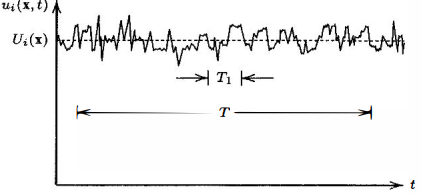
\includegraphics[width=0.5\textwidth]{foto01-decomposicao-reynolds.png}   
	\caption[Média temporal para turbulência estacionária para a velocidade instantânea $u_i(\textbf{x},t)$ \cite{Wilcox2006}]{Média temporal para turbulência estacionária para a velocidade instantânea $u_i(\textbf{x},t)$ \cite{Wilcox2006}.}
	\label{fig:decomposicao-reynolds}
\end{figure}

Como o foco da decomposição de Reynolds é resolver os problemas incompressíveis, as equações de Navier-Stokes para médias de Reynolds na forma conservativa são

\begin{gather}
	\label{eq:continuidade-decomposicao-reynolds}
	\frac{\partial U_i}{\partial x_i} = 0 \\
	\label{eq:momento-decomposicao-reynolds}
	\rho\frac{\partial U_i}{\partial t} + \rho\frac{\partial}{\partial x_j}\left(U_{j}U_{i} + \overline{u'_j u'_i} \right) = -\frac{\partial P}{\partial x_i} + \frac{\partial}{\partial x_j}\left(2\mu S_{ji}\right)
\end{gather}
%
o termo $S_{ij}$, presente na equação \ref{eq:momento-decomposicao-reynolds}, se trata do valor médio do tensor taxa de deformação, dado por

\begin{equation}
    \label{eq:tensor-medio-taxadeformacao}
    S_{ij} = \frac{1}{2}\left(\frac{\partial U_i}{\partial x_j} + \frac{\partial U_j}{\partial x_i} \right)
\end{equation}

O maior problema da turbulência é prescrever o termo $\overline{u'_{i}u'_{j}}$, mas ao reescrever a equação \ref{eq:momento-decomposicao-reynolds} conforme a equação RANS padrão \cite{Wilcox2006}:

\begin{equation}
	\rho\frac{\partial U_i}{\partial t} + \rho U_{j}\frac{\partial U_i}{\partial x_j} = -\frac{\partial P}{\partial x_i} + \frac{\partial}{\partial x_j}\left(2\mu S_{ji} - \rho\overline{u'_j u'_i} \right)
\end{equation}

A quantidade $-\rho\overline{u'_{i}u'_{j}}$ é conhecido por tensor tensão de Reynolds, também escrito como $\rho\tau_{ij}$, logo $\tau_{ij}$ é o tensor tensão de Reynolds específico dado por

\begin{equation}
	\tau_{ij} = -\overline{u'_j u'_i}
\end{equation}
%
onde se verifica que é um tensor simétrico ($\tau_{ij} = \tau_{ji}$) com 6 variáveis independentes e desconhecidas. Por esta razão, é preciso encontrar mais equações para fechar o sistema, que já possui 4 variáveis a serem calculadas num escoamento tridimensional, o que implica em assumir 10 equações ao todo.

\subsection{Decomposição de Favre}

Nos escoamentos compressíveis as variações de densidade do fluido não são desprezíveis com o gradiente de pressão, permitindo criar novos termos para as equações de governo. Para solucionar este problema, deve-se aplicar as decomposições de Favre (ou pela médias das massas). O procedimento visto em seu trabalho afirma que a propriedade pode ser vista como uma média no tempo ponderada pela densidade, definida como a equação \ref{eq:densidade-decomposicao-favre}

\begin{equation} 
	\label{eq:densidade-decomposicao-favre}
    \rho = \overline{\rho} + \rho'
\end{equation}

Introduzindo a velocidade média pela massa, $\Tilde{u}_i$, tem-se a equação \ref{eq:velocidade-decomposicao-favre}

\begin{equation}
	\label{eq:velocidade-decomposicao-favre}
	\Tilde{u_{i}} = \frac{1}{\overline{\rho}}\lim_{\tau \rightarrow \infty} \frac{1}{\tau}\int_{t}^{t+\tau}\rho(\textbf{x},t)u_i(\textbf{x},t)dt
\end{equation}
%
onde $\overline{\rho}$ é a densidade média da decomposição de Reynolds. Dentre as propriedades mais relevantes para as equações de conservação, a decomposição de Favre resulta nas seguintes expressões:

\begin{equation}
\left. \begin{aligned}
  u_i &= \tilde{u}_i + u''_i \\
  p &= P + p' \\
  h &= \Tilde{h} + h'' \\
  e &= \Tilde{e} + e'' \\
  T &= \Tilde{T} + T'' \\
  q_j & = q_{L_j} + q'_j
\end{aligned}
\right\rbrace
\end{equation}
%
as notações com til (ex: $\tilde{u}_i$) são médias pelas densidade, enquanto que as variáveis com $''$ (ex: $u''_i$) denotam as flutuações estatísticas geradas pelas médias de densidade. Logo abaixo estão as equações de governo para fluidos compressíveis de continuidade \ref{eq:continuidade-favre}, momento \ref{eq:momento-favre} e energia \ref{eq:energia-favre} que utilizam a decomposição de Favre \cite{Wilcox2006}:

\begin{gather}
    \label{eq:continuidade-favre}
    \frac{\partial \overline{\rho}}{\partial t} + \frac{\partial}{\partial x_i} \left( \overline{\rho} \Tilde{u}_{i}\right) = 0 \\
    \label{eq:momento-favre}
    \frac{\partial}{\partial t}\left(\overline{\rho} \Tilde{u_i} \right) + \frac{\partial}{\partial x_j} (\overline{\rho}\Tilde{u_i}\Tilde{u_j}) = -\frac{\partial P}{\partial x_i} + \frac{\partial}{\partial x_j}\left[\overline{t_{ji}} + \overline{\rho}\tau_{ji}\right] \\
    \label{eq:energia-favre} 
    \frac{\partial}{\partial t}\left(\overline{\rho}E\right) + \frac{\partial}{\partial x_j}(\overline{\rho} \Tilde{u_{j}} H) 
    = \frac{\partial}{\partial x_j}\left[-q_{L_{j}} - q_{T_{j}} + \overline{t_{ij}u''_i} - \overline{\rho u''_j\frac{1}{2}u''_i u''_i} \right] + \frac{\partial}{\partial x_j}\left[\Tilde{u_i}\left(\overline{t_{ij}} + \overline{\rho}\tau_{ij}\right)\right]
\end{gather}

Conforme nota-se ao longo do desenvolvimento das equações de Navier-Stokes, o termo P presente na equação \ref{eq:momento-favre} é a pressão corrigida para a decomposição de Favre, dada pela equação \ref{eq:pressao-favre}

\begin{equation}
	\label{eq:pressao-favre}
	P = \overline{\rho}R\Tilde{T}
\end{equation} 

Os termos $E$ e $H$ referem-se à energia total do sistema e a entalpia total do sistema, cujas equações demonstram ser funções da energia cinética turbulenta

\begin{equation}
	E = \Tilde{e} + \frac{1}{2}\Tilde{u_i}\Tilde{u_i} + \kappa 
	\hspace{0.5cm} 
	\text{e} 
	\hspace{0.5cm} 
	H = \Tilde{h} + \frac{1}{2}\Tilde{u_i}\Tilde{u_i} + \kappa
\end{equation} 

\subsubsection{Aproximações de Fechamento para os Escoamentos Compressíveis}

O fato de calcular as equações de Navier-Stokes a partir da decomposição de Favre resulta em resultados afetados pelos flutuações da densidade. Em qualquer modelo de transporte, aproximações de fechamento de caráter difusivo são normalmente postulados para as propriedades médias pela massa do tensor tensão de Reynolds e o vetor fluxo de calor \cite{Wilcox2006}. 

Para os modelos de zero até 2 equações, a hipótese de Boussinesq é uma razoável generalização dos escoamentos compressíveis, ou seja, o tensor tensão de Reynolds pela média das massas $\rho\tau_{ij}$ e a viscosidade dinâmica turbulenta $\mu_t$ é assumido da forma a seguir na equação \ref{eq:boussinesq-rans}

\begin{equation}
	\label{eq:boussinesq-rans}
	\rho\tau_{ij} \equiv \overline{-\rho u''_{i}u''_{j}} = 2\mu_t \left(S_{ij} - \frac{1}{3}\frac{\partial \Tilde{u}_k}{\partial x_k}\delta_{ij}\right) - \frac{2}{3}\overline{\rho}\kappa\delta_{ij}
\end{equation}

Outro termo que surgiu na equação \ref{eq:energia-favre} é o vetor fluxo turbulento de calor, $q_{T_j}$, cuja aproximação para o fechamento foi proposta por Reynolds (1874), que assume ser proporcional ao gradiente médio de temperatura, como visto na equação \ref{eq:fluxo-turbulento-calor-reynolds} 

\begin{equation}
	\label{eq:fluxo-turbulento-calor-reynolds}
	q_{T_j} = \overline{\rho u''_j h''} = -\frac{\mu_t c_p}{Pr_t}\frac{\partial \tilde{T}}{\partial x_j} = -\frac{\mu_t}{Pr_t}\frac{\partial \tilde{h}}{\partial x_j}
\end{equation}
%
onde $Pr_t$ é o número de Prandtl turbulento, que costuma ser aplicado como uma constante nos modelos RANS de turbulência \cite{Wilcox2006}.

\section{Modelo Spalart-Allmaras}

Esse modelo \cite{Spalart1992} envolve uma equação de transporte para a viscosidade cinética turbulenta ($\nu_t$). É amplamente utilizado em estudos sobre camadas-limites em projetos aerodinâmicos. O objetivo da aplicação deste modelo é possibilitar resultados prévios com alguma precisão ao menor custo computacional. Este método desejava remover as incompletudes dos modelos algébricos para cálculo da turbulência e, ao mesmo tempo, ser computacionalmente mais simples do que os modelos com duas equações \cite{pope_2000}. A viscosidade turbulenta é aplicada da forma vista na equação \ref{eq:visc-sa}:

\begin{equation}
    \label{eq:visc-sa}
    \nu_t = \Tilde{\nu} f_{\nu 1} \hspace{5mm} f_{\nu 1} = \frac{\chi^3}{\chi^3 + c^{3}_{\nu 1}} \hspace{5mm} \chi = \frac{\Tilde{\nu}}{\nu}
\end{equation}

E $\Tilde{\nu}$ obedece a equação de transporte \ref{eq22:transport-sa}

\begin{equation}\label{eq22:transport-sa}
\begin{split}
    \frac{D\Tilde{\nu}}{Dt} &= c_{b1}[1 - f_{t2}]\Tilde{S}\Tilde{\nu} + \frac{1}{\sigma}\left[\nabla \cdot ((\nu + \Tilde{\nu})\nabla \Tilde{\nu}) + c_{b2}(\nabla \Tilde{\nu})^2 \right] \\&- \left[c_{w1}f_w - \frac{c_{b1}}{\kappa^2}f_{t2}\right]\left[\frac{\nu}{d}\right]^2 + f_{t1}\Delta U^2
\end{split}
\end{equation}

Considerando que

\begin{equation}
    \Tilde{S} \equiv S + \frac{\Tilde{\nu}}{\kappa^2d^2}f_{v2} \hspace{5mm} f_{v2} = 1 - \frac{\chi}{1 + \chi f_{v1}}
\end{equation}

Onde $S$ é a vorticidade e $d$ a distância até a parede mais próxima. Já a função $f_{w}$ é dada por

\begin{equation}
    f_w = g\left[\frac{1 + c^{6}_{w3}}{g^6 + c^{6}_{w3}} \right]^{1/6} \hspace{5mm} g = r + c_{w2}(r^6 - r) \hspace{5mm} r \equiv \frac{\Tilde{\nu}}{\Tilde{S}\kappa^2d^2}
\end{equation}

Pode-se assumir $f_w = 10$ quando r é um valor grande. Enquanto isso, a função $f_{t2}$ é dada por

\begin{equation}
    f_{t2} = c_{t3}\exp{(-c_{t4}\chi^2)}
\end{equation}

A última função $f_{t1}$ que aparece na equação \ref{eq22:transport-sa} pode ser deduzida da forma a seguir:

\begin{equation}
    \label{eq:ft1-sa}
    f_{t1} = c_{t1}g_{t} \exp{\left(-c_{t2}\frac{\omega_{t}^{2}}{\Delta U^2}\left[d^{2} + g_{t}^{2}d_{t}^{2}\right]\right)} \hspace{5mm} g_t \equiv min(0,1, \Delta U/\omega_t \Delta x_t)
\end{equation}

onde $\Delta x_t$ é o espaçamento ao longo da malha. As constantes utilizadas das equações \ref{eq:visc-sa} até \ref{eq:ft1-sa} podem ser vistas na Tabela \ref{tab:tabela-constantes-spalart-allmaras}. Os resultados obtidos mostraram a baixa influência da variação de densidade ao estudar os regimes supersônico \cite{Spalart1992}.

\begin{table}[ht]
\centering
\caption[Constantes usadas no modelo Spalart-Allmaras \cite{Spalart1992}]{Constantes usadas no modelo Spalart-Allmaras \cite{Spalart1992}}
\vspace{0.5cm}
\begin{tabular}{c|c}
 
Constante & Valor \\
\hline
$c_{b1}$ & 0,1355 \\
$\sigma$ & 2/3 \\
$c_{b2}$ & 0,622 \\
$\kappa$ & 0,41 \\
$c_{w1}$ & $c_{b1}/\kappa$ + (1 + $c_{b2}$)/$\sigma$ \\
$c_{w2}$ & 0,3 \\
$c_{w3}$ & 2,0 \\
$c_{\nu 1}$ & 7,1 \\
$c_{t1}$ & 1,0 \\
$c_{t2}$ & 2,0 \\
$c_{t3}$ & 1,2 \\
$c_{t4}$ & 0,5 \\

\end{tabular}
\label{tab:tabela-constantes-spalart-allmaras}
\fonte{\cite{Spalart1992}}
\end{table}

\section{Modelo \texorpdfstring{$\kappa$-$\varepsilon$}{k-e} Padrão}

O modelo $\kappa$-$\varepsilon$ \cite{JONES1972301,LAUNDER1974269,launder1974} apresenta uma forma de compreender a viscosidade turbulenta local através da energia cinética turbulenta ($\kappa$) e pela taxa de dissipação dessa energia por unidade de massa ($\varepsilon$). A viscosidade cinemática turbulenta ($\nu_t$) é apresentada abaixo na equação \ref{eq:nut-k-epsilon}

\begin{equation}
    \nu_t = \frac{C_\mu k^2}{\varepsilon}
    \label{eq:nut-k-epsilon}
\end{equation}

Em altos números de Reynolds, as propriedades envolvidas possuem suas equações de transporte para a energia cinética turbulenta \ref{eq:transporte-k-modelo-k-epsilon} e para a taxa de dissipação específica \ref{eq:transporte-eps-modelo-k-epsilon} a serem resolvidas \cite{Wilcox2006}

\begin{gather}
    \frac{\partial \kappa}{\partial t} + U_{j} \frac{\partial \kappa}{\partial x_j} = \tau_{ij}\frac{\partial U_i}{\partial x_j} - \varepsilon + \frac{\partial}{\partial x_j}\left[\left(\nu + \nu_{t}/\sigma_{\kappa}\right)\frac{\partial \kappa}{\partial x_j}\right]
    \label{eq:transporte-k-modelo-k-epsilon}
    \\
   	\frac{\partial \varepsilon}{\partial t} + U_{j} \frac{\partial \varepsilon}{\partial x_j} = C_{1}\frac{\varepsilon}{\kappa}\tau_{ij}\frac{\partial U_i}{\partial x_j} - C_{2}\frac{\varepsilon^{2}}{\kappa} + \frac{\partial}{\partial x_j}\left[\left(\nu + \nu_{t}/\sigma_{\varepsilon}\right)\frac{\partial \varepsilon}{\partial x_j}\right]
    \label{eq:transporte-eps-modelo-k-epsilon}
\end{gather}
	
As constantes utilizadas neste método foram obtidas a partir de testes experimentais \cite{JONES1972301}, cujos resultados são apresentados na \autoref{tab:tabela-constantes-k-epsilon}. Embora o presente modelo seja bastante utilizado e obtenha bons resultados para escoamentos simples com gradientes de pressão considerados pequenos, o mesmo possui imprecisão nas proximidades de gradientes de pressão adversos \cite{Wilcox1988ReassessmentOT}. Portanto, há uma restrição deste modelo para análise de camada limite, a não ser que aplique um tratamento para amortecer a viscosidade turbulenta nessa região em que o número de Reynolds é baixo \cite{Moukalled2015}.

\begin{table}[ht]
\centering
\caption[Constantes usadas no modelo $\kappa$-$\varepsilon$ \cite{JONES1972301}]{Constantes usadas no modelo $\kappa$-$\varepsilon$ \cite{JONES1972301}}
\vspace{0.5cm}
\begin{tabular}{c|c}
 
Constante & Valor \\
\hline
$C_{\mu}$ & 0,09 \\
$C_{1}$ & 1,44 \\
$C_{2}$ & 1,92 \\
$\sigma_{k}$ & 1,0 \\
$\sigma_{\varepsilon}$ & 1,3

\end{tabular}
\label{tab:tabela-constantes-k-epsilon}
\fonte{\cite{JONES1972301}}
\end{table}

\section{Modelo \texorpdfstring{$\kappa$-$\omega$}{k-w} Padrão}

O modelo $\kappa$-$\omega$ padrão \cite{Wilcox1988ReassessmentOT,Wilcox2006,Wilcox2008} constata as dificuldades do modelo $\kappa$-$\varepsilon$ em predizer as camadas limites em gradientes adversos de pressão. A aplicação da lei da parede tende a esconder as imperfeições desses métodos. As análises feitas pelo desenvolvedor deste modelo permitiram-no concluir que a abordagem $\kappa$-$\omega$ é satisfatória em escoamentos compressíveis, seja na camada limite ou em meio livre. Partindo da mesma sequência feita no modelo anterior, a viscosidade cinemática turbulenta ($\nu_t$) é apresentada abaixo na equação \ref{eq:nu_t&kt_k-omega}.

\begin{equation}
    \nu_t = \frac{k}{\tilde{\omega}}
   	\hspace{1.0cm}
    \tilde{\omega} = \max{\left\lbrace \omega, C_{lim}\sqrt{\frac{2 S_{ij}S_{ij}}{\beta^*}}\right\rbrace}
    \hspace{1.0cm}
    C_{lim} = \frac{7}{8}
    \label{eq:nu_t&kt_k-omega}
\end{equation}

Mesmo sem fatores de amortecimento para a viscosidade turbulenta ou o uso da lei da parede, os resultados foram satisfatórios para estudos sobre a região da subcamada viscosa dentro da camada limite. Em adição aos fatos, os estudos também foram precisos em superfícies rugosas ou em escoamentos com adição de massa. Considerando $\omega$ como a taxa específica de dissipação da energia, ela é definida pela equação \ref{eq:omega-k-omega}

\begin{equation}
	\label{eq:omega-k-omega}
	\omega = \frac{\varepsilon}{\beta^{*}\kappa}
\end{equation}

As vantagens de escolher esse modelo em vez do $\kappa-\varepsilon$ padrão são \cite{Moukalled2015}:

\begin{enumerate}

	\item Mais robusto, por ser mais fácil de integrar numericamente;
	
	\item Pode ser integrado na região da subcamada limite viscosa sem aplicar funções de parede;

	\item Performa melhor com baixo gradiente adverso de pressão.
	
\end{enumerate}

As equações de transporte para a energia cinética turbulenta ($\kappa$) \ref{eq:transporte-k-modelo-k-omega} e para a taxa específica de dissipação de energia ($\omega$) \ref{eq:transporte-w-modelo-k-omega} são apresentadas abaixo \cite{Wilcox1988ReassessmentOT,Wilcox2006,Wilcox2008}

\begin{gather}
    \frac{\partial\rho\kappa}{\partial t} + \frac{\partial \rho u_{j}\kappa}{\partial x_j} = \rho\tau_{ij}\frac{\partial u_i}{\partial x_j} - \beta^{*}\rho\kappa\omega + \frac{\partial}{\partial x_j}\left[\left(\mu + \sigma^{*}\frac{\rho\kappa}{\omega}\right)\frac{\partial\kappa}{\partial x_j}\right]
    \label{eq:transporte-k-modelo-k-omega}
    \\
   	\frac{\partial \rho\omega}{\partial t} + \frac{\partial\rho u_j\omega}{\partial x_j} = \alpha\frac{\omega}{\kappa}\rho\tau_{ij}\frac{\partial u_i}{\partial x_j} - \beta\rho\omega^{2} + \sigma_{d}\frac{\rho}{\omega}\frac{\partial\kappa}{\partial x_j}\frac{\partial\omega}{\partial x_j} + \frac{\partial}{\partial x_j}\left[\left(\mu + \sigma\frac{\rho\kappa}{\omega}\right)\frac{\partial\omega}{\partial x_j}\right]
    \label{eq:transporte-w-modelo-k-omega}
\end{gather}

As relações auxiliares para calcular o modelo são descritas a seguir:

\begin{equation}
\begin{aligned}
	\beta = \beta_{0}f_{\beta} 
	\hspace{1cm}
	\sigma_{d} =
	\begin{cases}
		0, &	\frac{\partial\kappa}{\partial x_j	}\frac{\partial \omega}{\partial x_j} \leq 0 \\
		\sigma_d, & \frac{\partial\kappa}{\partial x_j	}\frac{\partial \omega}{\partial x_j} > 0
	\end{cases}
	\hspace{1cm}
	f_{\beta} = \frac{1 + 85\chi_{\omega}}{1 + 100\chi_{\omega}} \\
	\chi_{\omega} \equiv \left|\frac{\Omega_{ij}\Omega_{ij}\hat{S}_{ki}}{(\beta^{*}\omega)^3}\right|
	\hspace{1cm}
	\Omega_{ij} = \frac{1}{2}\left(\frac{\partial U_i}{\partial x_j} - \frac{\partial U_j}{\partial x_i}\right)
	\hspace{1cm}
	\hat{S}_{ki} = S_{ki} - \frac{1}{2}\frac{\partial u_m}{\partial x_m}\delta_{ki}
\end{aligned}
\end{equation}

O maior contraponto a este modelo é a sensibilidade aos valores especificados para o escoamento livre \cite{Menter1992}, o que leva a forte dependência da solução arbitrária de $\omega$ no meio livre, o que já não acontece no modelo $\kappa-\varepsilon$. Os coeficientes utilizados no modelo $\kappa$-$\omega$ são fornecidos na \autoref{tab:tabela-constantes-k-omega}

\begin{table}[ht]
\centering
\caption[Constantes usadas no modelo $\kappa$-$\omega$ \cite{Wilcox1988ReassessmentOT,Wilcox2006,Wilcox2008}]{Constantes usadas no modelo $\kappa$-$\omega$ \cite{Wilcox1988ReassessmentOT,Wilcox2006,Wilcox2008}}
\vspace{0.5cm}
\begin{tabular}{c|c}
 
Constante & Valor \\
\hline
$\alpha$ & 13/25 \\
$\beta^*$ & 0,09 \\
$\beta_{0}$ & 0,0708 \\
$\sigma$ & 1/2 \\
$\sigma^*$ & 3/5 \\
$\sigma_{do}$ & 1/8

\end{tabular}
\label{tab:tabela-constantes-k-omega}
\fonte{\cite{Wilcox1988ReassessmentOT,Wilcox2006,Wilcox2008}}
\end{table}

\section{Modelo \textit{Shear Stress Transport} \texorpdfstring{$\kappa$-$\omega$}{k-w}}

O modelo SST k-$\omega$ \cite{Menter1994TwoequationET,Menter2003,Menter2009} é baseado em duas equações para descrever a viscosidade turbulenta. Durante o desenvolvimento do modelo, muitos testes experimentais foram realizados, com ênfase em projetos aerodinâmicos. Foi proposto para as simulações de escoamentos aeronáuticos com altos gradientes adversos de pressão e separação de camada limite, por meio de uma combinação dos modelos $\kappa$-$\varepsilon$ e $\kappa$-$\omega$.

Com respeito a casos de escoamentos com camada limite, o modelo $\kappa$-$\omega$ apresenta melhores resultados que o modelo $\kappa$-$\varepsilon$ na solução da região viscosa próxima a parede, e seus resultados tem sido satisfatórios em casos que envolvem gradientes de pressão adversos. Entretanto, o modelo $\kappa$-$\omega$ exige uma condição de contorno não nula para $\omega$ para correntes livres não turbulentas, e o fluxo calculado apresenta elevada sensibilidade ao valor especificado \cite{Menter1994TwoequationET}. Foi demonstrado que o modelo $\kappa$-$\varepsilon$ não apresenta essa deficiência \cite{Cazalbou1994}.

Logo, o modelo SST $\kappa$-$\omega$ trata-se da combinação robusta e precisa do modelo $\kappa$-$\omega$ na região próxima das paredes com a independência da corrente livre do modelo $\kappa$-$\varepsilon$ fora da camada limite. Para isso, o modelo $\kappa$-$\varepsilon$ é escrito em termos da taxa de dissipação específica, $\omega$. Em seguida, o modelo $\kappa$-$\omega$ padrão e o modelo $\kappa$-$\varepsilon$ modificado são multiplicados por uma função de mistura e somados. As equações de transporte são desenvolvidas como a seguir em \ref{eq:transporte-k-modelo-sst-k-omega} e \ref{eq:transporte-w-modelo-sst-k-omega}.

\begin{gather}
    \frac{\partial}{\partial t}(\rho\kappa) +\frac{\partial}{\partial x_i}(\rho u_i \kappa) = \tilde{P}_\kappa - \beta^{*}\rho\kappa\omega + \frac{\partial}{\partial x_i}\left[(\mu + \sigma_{\kappa}\mu_t)\frac{\partial \kappa}{\partial x_i}\right]
    \label{eq:transporte-k-modelo-sst-k-omega}
    \\
   	\frac{\partial}{\partial t}(\rho\omega) +\frac{\partial}{\partial x_i}(\rho u_i \omega)  = \alpha\frac{1}{\nu_t}\tilde{P}_\kappa - \beta\rho\omega^{2} + \frac{\partial}{\partial x_i}\left[(\mu + \sigma_{\omega}\mu_t)\frac{\partial \omega}{\partial x_i}\right] + 2(1 - F_1)\rho\sigma_{w2}\frac{1}{\omega}\frac{\partial\kappa}{\partial x_i}\frac{\partial \omega}{\partial x_i}
    \label{eq:transporte-w-modelo-sst-k-omega}
\end{gather}
%
cujos coeficientes dos modelos $\kappa-\varepsilon$ e $\kappa-\omega$ dependem da função de mistura $F_1$, que é obtido pela equação \ref{eq:funcaomistura-modelo-sst-k-omega}

\begin{equation}
	\label{eq:funcaomistura-modelo-sst-k-omega}
    \tilde{\Gamma} = F_1 \Gamma_1 + (1 - F_1) \Gamma_2
\end{equation}
%
onde 

\begin{equation}
		F_1 = \tanh{(arg_1^{4})}
		\hspace{1cm}
    	arg_1 = \min\left[\max\left(\frac{\sqrt{\kappa}}{\beta^{*}\omega d(\perp)};\frac{500\nu}{d(\perp)^2 \omega}\right);\frac{4\rho\sigma_{\omega 2}\kappa}{CD_{k\omega}d(\perp)^2}\right]
\end{equation}
%
considere que $d(\perp)$ é a distância perpendicular mais próxima à superfície e $CD_{k\omega}$ é a parte positiva do termo de difusão cruzada.

\begin{equation}
    CD_{k\omega} = \max\left(2\rho\sigma_{\omega 2}\frac{1}{\omega}\frac{\partial \kappa}{\partial x_j}\frac{\partial \omega}{\partial x_j}, 10^{-10} \right)
\end{equation}

Neste modelo há uma relação que satisfaz a relação de Bradshaw, que apresenta a equação \ref{eq:bradshaw-tensao-k} para correlacionar as tensões principais, $\tau_{xy}$, com a energia cinética turbulenta \cite{Menter1994TwoequationET}.

\begin{equation}
	\label{eq:bradshaw-tensao-k}
	\tau_{xy} = \mu_{t}\Omega = \rho\sqrt{\frac{\text{Produção de }\kappa}{\text{Dissipação de }\kappa}}a_{1}\kappa
\end{equation}

Assumindo que $\Omega$ é a vorticidade, dada pela seguinte equação \ref{eq:vorticidade-modelo-sst-k-omega}.

\begin{equation}
	\label{eq:vorticidade-modelo-sst-k-omega}
	\Omega = \sqrt{2 S_{ij}S_{ij}}
\end{equation}

Para a viscosidade cinemática turbulenta $\nu_t$, a equação \ref{eq:visc-sst} é dada por

\begin{equation}
\begin{split}
    \label{eq:visc-sst}
    \nu_t = \frac{a_1 \kappa}{\max(a_1 \omega;\Omega F_2)} \hspace{1cm}
    F_2 = \tanh{\left(\max\left(2\frac{\sqrt{\kappa}}{\beta^{*}\omega d(\perp)}; \frac{500\nu}{ d(\perp)^2\omega}\right)^{2}\right)} 
\end{split}
\end{equation}
%
onde $a_1 = 0,31$. O termo $\tilde{P}_{\kappa}$ também significa a produção de energia cinética turbulenta, mas usada neste modelo para prevenir o crescimento da turbulência em regiões de estagnação \cite{Menter2009}. A equação \ref{eq:producao-tilde-k-modelo-sst-k-omega} se refere a esse ajuste do modelo SST

\begin{equation}
	\label{eq:producao-tilde-k-modelo-sst-k-omega}
	P_{\kappa} = \mu_{t}\frac{\partial u_i}{\partial x_j}\left(\frac{\partial u_i}{\partial x_j} + \frac{\partial u_j}{\partial x_i}\right)
	\hspace{1cm}
	\tilde{P}_{\kappa} = \min(P_\kappa, 10\cdot\beta^{*}\rho\kappa\omega)
\end{equation}

Houve uma ligeira alteração na primeira versão deste modelo RANS \cite{Menter1994TwoequationET}, pois o $\tilde{P}_{\kappa}$ era proposto num fator de 20 em vez de 10. A \autoref{tab:tabela-constantes-SST-k-omega} apresenta as constantes utilizadas para a formulação deste modelo de 2 equações:

\begin{table}[ht]
\centering
\caption[Constantes usadas no modelo SST $\kappa$-$\omega$ \cite{Menter1994TwoequationET,Menter2003,Menter2009}]{Constantes usadas no modelo SST $\kappa$-$\omega$ \cite{Menter1994TwoequationET,Menter2003,Menter2009}}
\vspace{0.5cm}
\begin{tabular}{c|c|c|c}
 
Constante ($\Gamma_1$) & Valor & Constante ($\Gamma_2$) & Valor \\
\hline
$\alpha_1$ & 0,5532 & $\alpha_2$ & 0,4403 \\
$\beta_1$ & 0,075 & $\beta_2$ & 0,0828 \\
$\sigma_{\kappa 1}$ & 0,85 & $\sigma_{\kappa 2}$ & 1,0 \\
$\sigma_{\omega 1}$ & 0,50 & $\sigma_{\omega 2}$ & 0,856 \\
$\beta^{*}$ & 0,09 & $\beta^{*}$ & 0,09 \\
$k$ & 0,41 & $k$ & 0,41

\end{tabular}
\label{tab:tabela-constantes-SST-k-omega}
\fonte{\cite{Menter1994TwoequationET,Menter2003,Menter2009}}
\end{table}

O modelo SST $\kappa$-$\omega$ levou a uma grande melhoria, se comparado aos modelos $\kappa$-$\omega$ e $\kappa$-$\varepsilon$, para todos os escoamentos que envolvem gradientes adversos de pressão e \citeauthor{Menter1994TwoequationET} sugere que seja a técnica mais utiliza quando se trata de problemas de aerodinâmica. Outro fato importante é que nenhum outro método de duas equações para descrever a turbulência conseguiu predizer com acurácia a separação da pressão induzida e a interação viscosa-invíscida do escoamento.